\chapter{Исследовательская часть}

В данном разделе приведены графовые модели алгоритмов реализующих вывод всех целых чисел в диапазоне от $A$ до $B$ включительно при условии $A \leqslant B$. В рекурсивном алгоритме для рекурсивного вызова используется вершина 5, а 5б для присваивание его результата переменной.

Вершины графа представляют собой строчки кода представленного в листингах~\ref{lst:recursive}~---\ref{lst:iterative}

\section{Граф управления}
Граф управления рекурсивного алгоритма приведен на рисунке~\ref{fig:shemanum3}.  

\begin{figure}[h!]
	\centering
	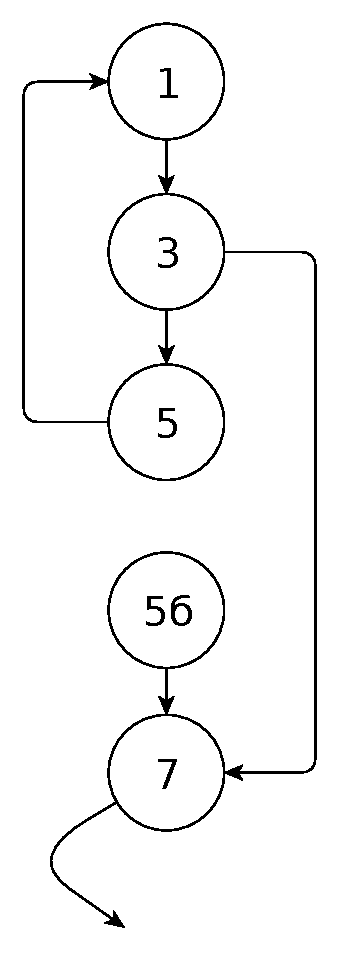
\includegraphics[width=0.3\textwidth]{images/shema_num3}
	\caption{Граф управления рекурсивного алгоритма}
	\label{fig:shemanum3}
\end{figure}


\clearpage


На рисунке~\ref{fig:shemanum4} приведен граф управления итеративного алгоритма. 


\begin{figure}[h!]
	\centering
	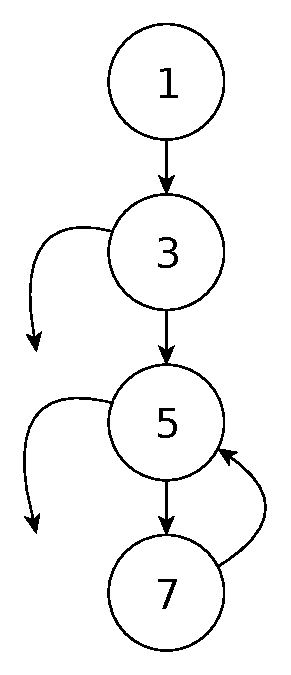
\includegraphics[width=0.3\textwidth]{images/shema_num4}
	\caption{Граф управления итеративного алгоритма}
	\label{fig:shemanum4}
\end{figure}


\clearpage

\section{Информационный граф}

На рисунке~\ref{fig:shemanum5} приведен информационный граф рекурсивного алгоритма

\begin{figure}[h!]
	\centering
	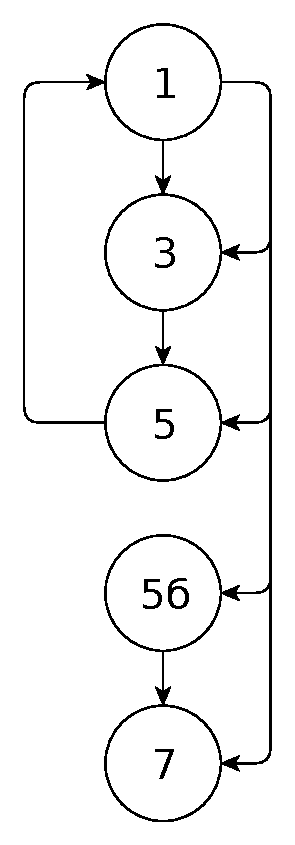
\includegraphics[width=0.3\textwidth]{images/shema_num5}
	\caption{Информационный граф рекурсивного алгоритма}
	\label{fig:shemanum5}
\end{figure}

\clearpage
На рисунке~\ref{fig:shemanum6} приведен информационный граф итеративного алгоритма

\begin{figure}[h!]
	\centering
	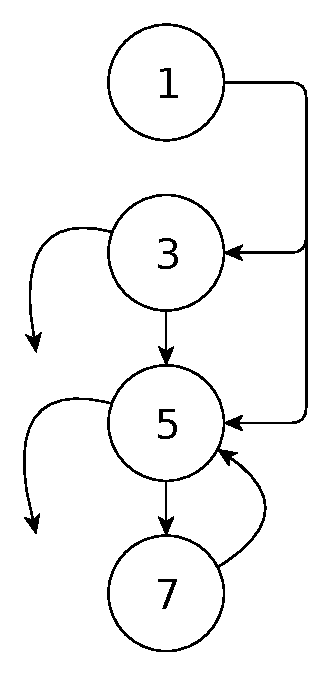
\includegraphics[width=0.3\textwidth]{images/shema_num6}
	\caption{Информационный граф итеративного алгоритма}
	\label{fig:shemanum6}
\end{figure}

\clearpage

\section{Операционная история}

Для построения операционной истории рекурсивного алгоритма в качестве входных данных использовались значения $A = 1$ и $B = 7$

На рисунке~\ref{fig:shemanum7} приведена операционная история рекурсивного алгоритма

\begin{figure}[h!]
	\centering
	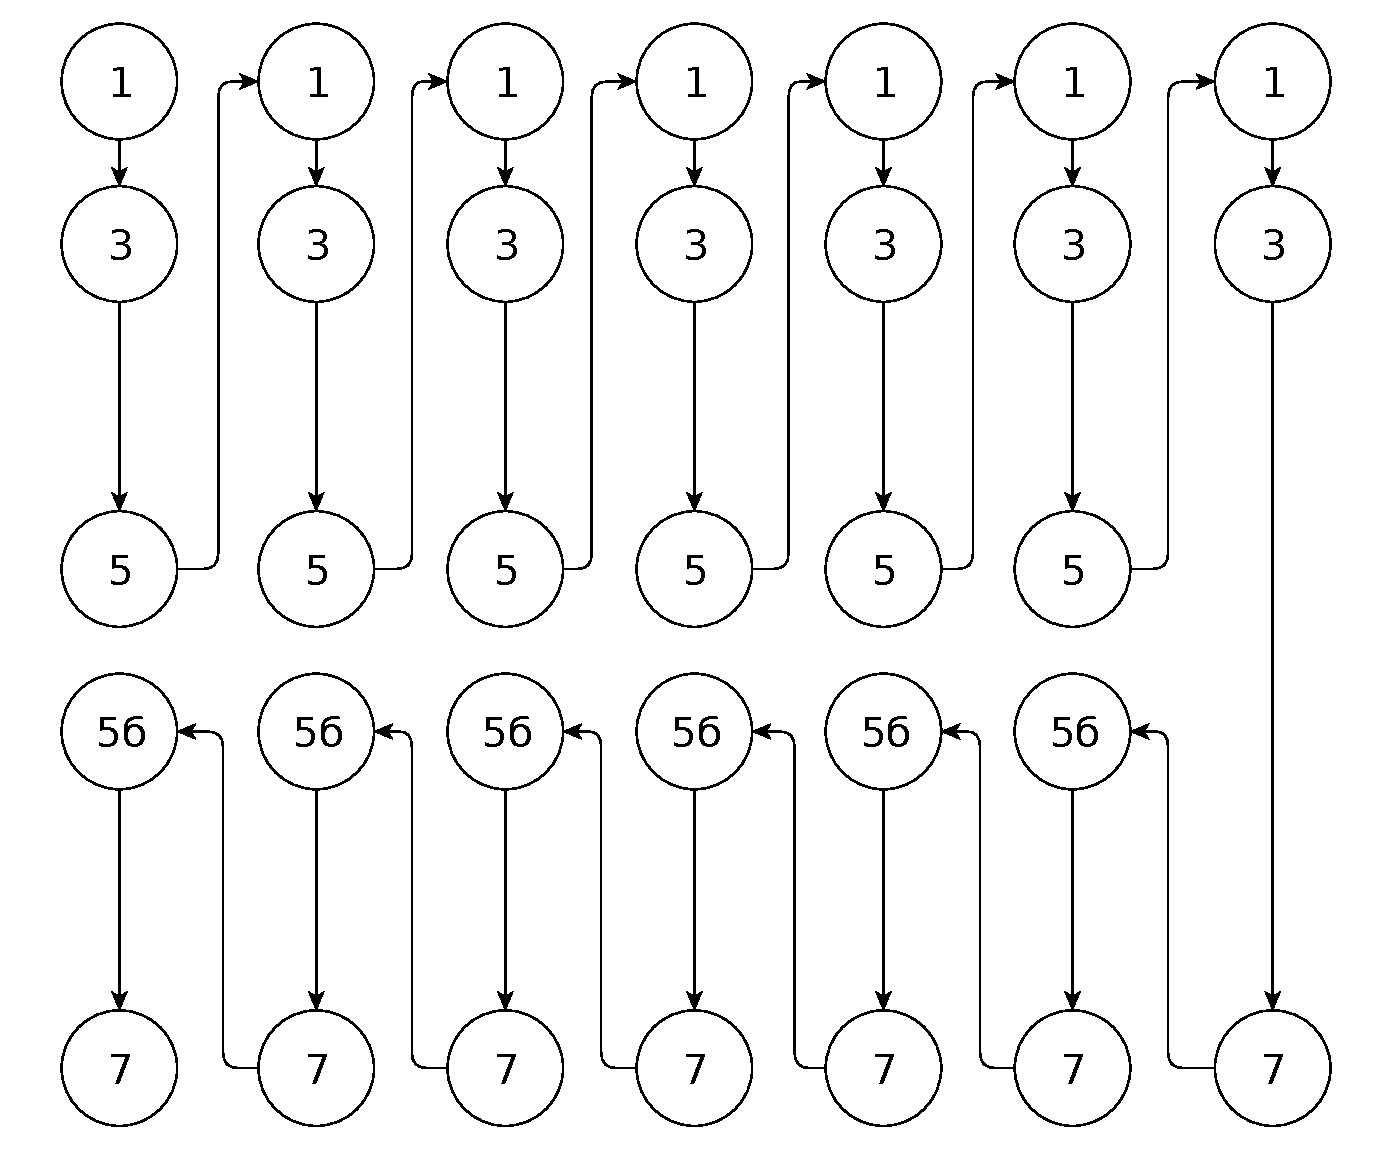
\includegraphics[width=1\textwidth]{images/shema_num7}
	\caption{Операционная история рекурсивного алгоритма}
	\label{fig:shemanum7}
\end{figure}

\clearpage
Для построения операционной истории итеративного алгоритма в качестве входных данных использовались значения $A = 1$ и $B = 6$

На рисунке~\ref{fig:shemanum8} приведена операционная история итеративного алгоритма

\begin{figure}[h!]
	\centering
	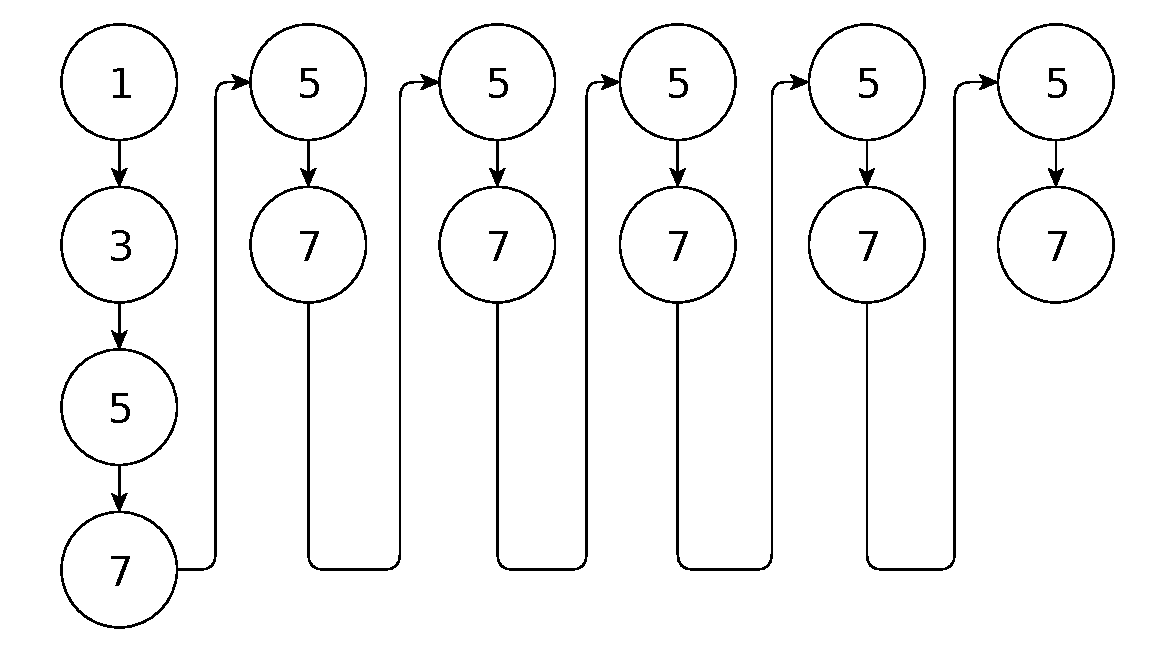
\includegraphics[width=1\textwidth]{images/shema_num8}
	\caption{Операционная история итеративного алгоритма}
	\label{fig:shemanum8}
\end{figure}

\section{Информационная история}

Для построения информационной истории рекурсивного алгоритма в качестве входных данных использовались значения $A = 1$ и $B = 7$

На рисунке~\ref{fig:shemanum9} приведена информационная история рекурсивного алгоритма

\begin{figure}[h!]
	\centering
	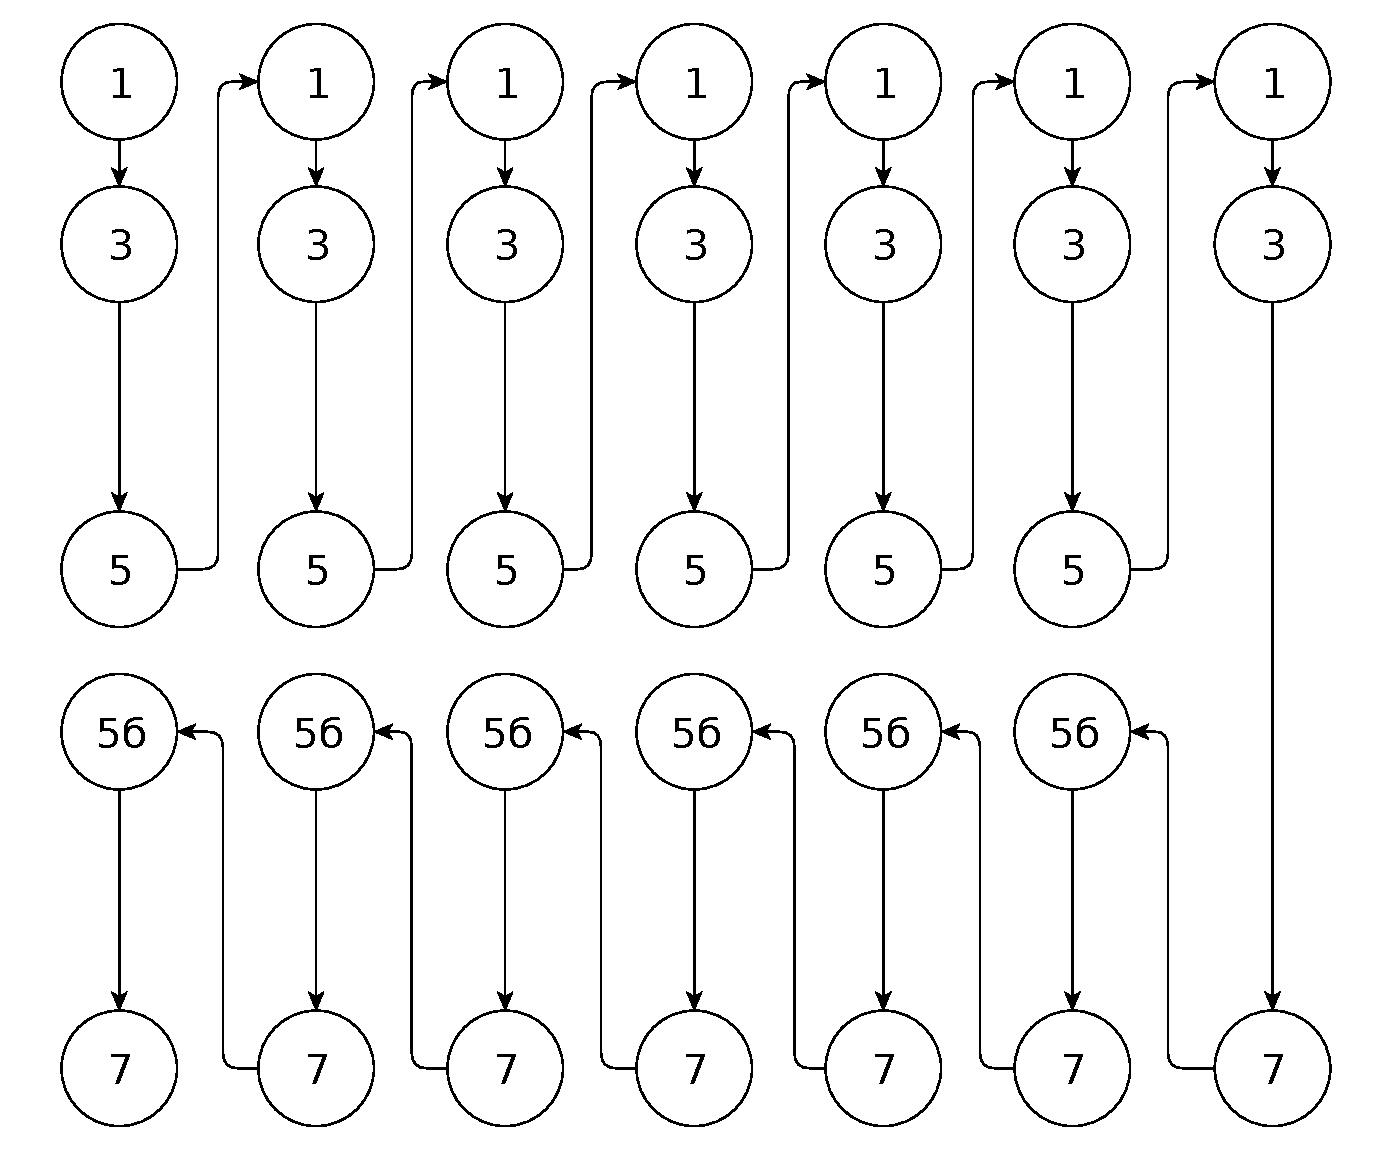
\includegraphics[width=1\textwidth]{images/shema_num9}
	\caption{Информационная история рекурсивного алгоритма}
	\label{fig:shemanum9}
\end{figure}

\clearpage

Для построения информационной истории итеративного алгоритма в качестве входных данных использовались значения $A = 1$ и $B = 6$

На рисунке~\ref{fig:shemanum10} приведена информационная история рекурсивного алгоритма

\begin{figure}[h!]
	\centering
	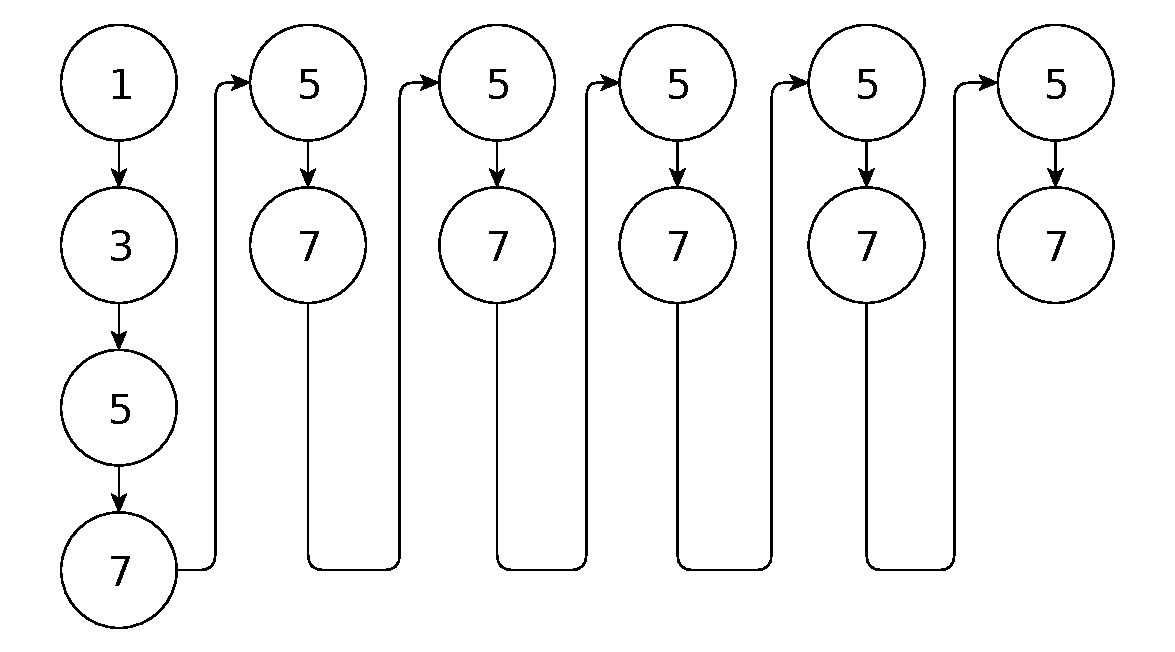
\includegraphics[width=1\textwidth]{images/shema_num10}
	\caption{Информационная история итеративного алгоритма}
	\label{fig:shemanum10}
\end{figure}

\section{Вывод}
Проведённый анализ графовых моделей рекурсивного и итеративного алгоритмов показал отсутствие шагов, допускающих параллельное выполнение. Все вершины графов соединены между собой через информационные или операционные зависимости.
